\subsubsection{Q10.20 data 09202021 10082021 grouped by scenario}

\begin{comment}
           EFPR   EO      EFNR     n    pvalue
(frauth,)   0.5  0.5  0.500000  34.0  1.000000
(icu,)      0.5  0.5  0.607143  28.0  0.896890
(rent,)     0.5  0.5  0.378788  33.0  0.912596
\end{comment}

\begin{table}[h]
    \centering
    \begin{tabular}{|c|c|c|c|c|c|}
        \hline
        scenario & EFPR & EO & EFNR & n & p-value\\
        \hline
        frauth & 0.500 & 0.500 & 0.500 & 34.0 & 1.000\\
		icu & 0.500 & 0.500 & \textbf{0.607} & 28.0 & 0.897\\
		rent & 0.500 & 0.500 & 0.379 & 33.0 & 0.913\\
		
        \hline
    \end{tabular}
    \caption{Grouped by scenario}
    \label{tab:my_label}
\end{table}
\begin{figure}[h]
    \centering
    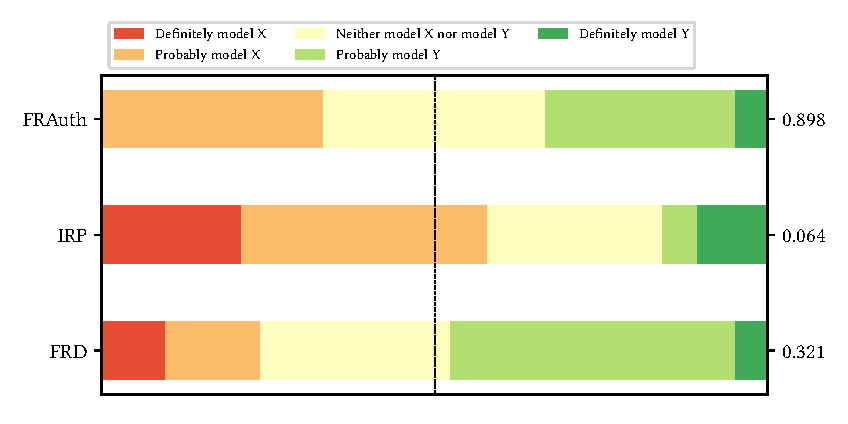
\includegraphics[width=0.8\textwidth]{figures/Q10.20/09202021_10082021/Q10.20_scenario.pdf}
    \caption{Grouped by scenario}
    \label{fig:my_label}
\end{figure}
